\documentclass[11pt]{article}

\usepackage{float}
\usepackage{multicol}
\usepackage{graphicx}
\usepackage{hyperref}
\hypersetup
{
    colorlinks=true,
    linkcolor=black,
    filecolor=blue,      
	urlcolor=blue,
	citecolor=black
}

\title{Machine Learning -- Homework 2}
\author{Andrea Gasparini \\ \texttt{1813486}}
\date{December 2020}

\begin{document}
	\maketitle
	\tableofcontents
	\newpage

	\section{Introduction}
	The goal of this Homework was to solve an image classification problem with
	objects typically available in a home environment.



	\section{Dataset}
	The dataset contains \textbf{8221} samples and it's based on a 8 classes subset of the
	\href{https://sites.google.com/diag.uniroma1.it/robocupathome-objects/home}{RoboCup@Home-Objects dataset}.
	For each class we have a folder containing all the related samples.

	\begin{multicols}{2}
		\begin{itemize}
			\item \textit{accent plate}
			\item \textit{breadsticks}
			\item \textit{cereals box}
			\item \textit{cocoa drink bottle}
			\item \textit{nitrile gloves}
			\item \textit{paper bag}
			\item \textit{pears}
			\item \textit{plastic fork}
		\end{itemize}
	\end{multicols}	

	\begin{figure}[H]
		\centering
		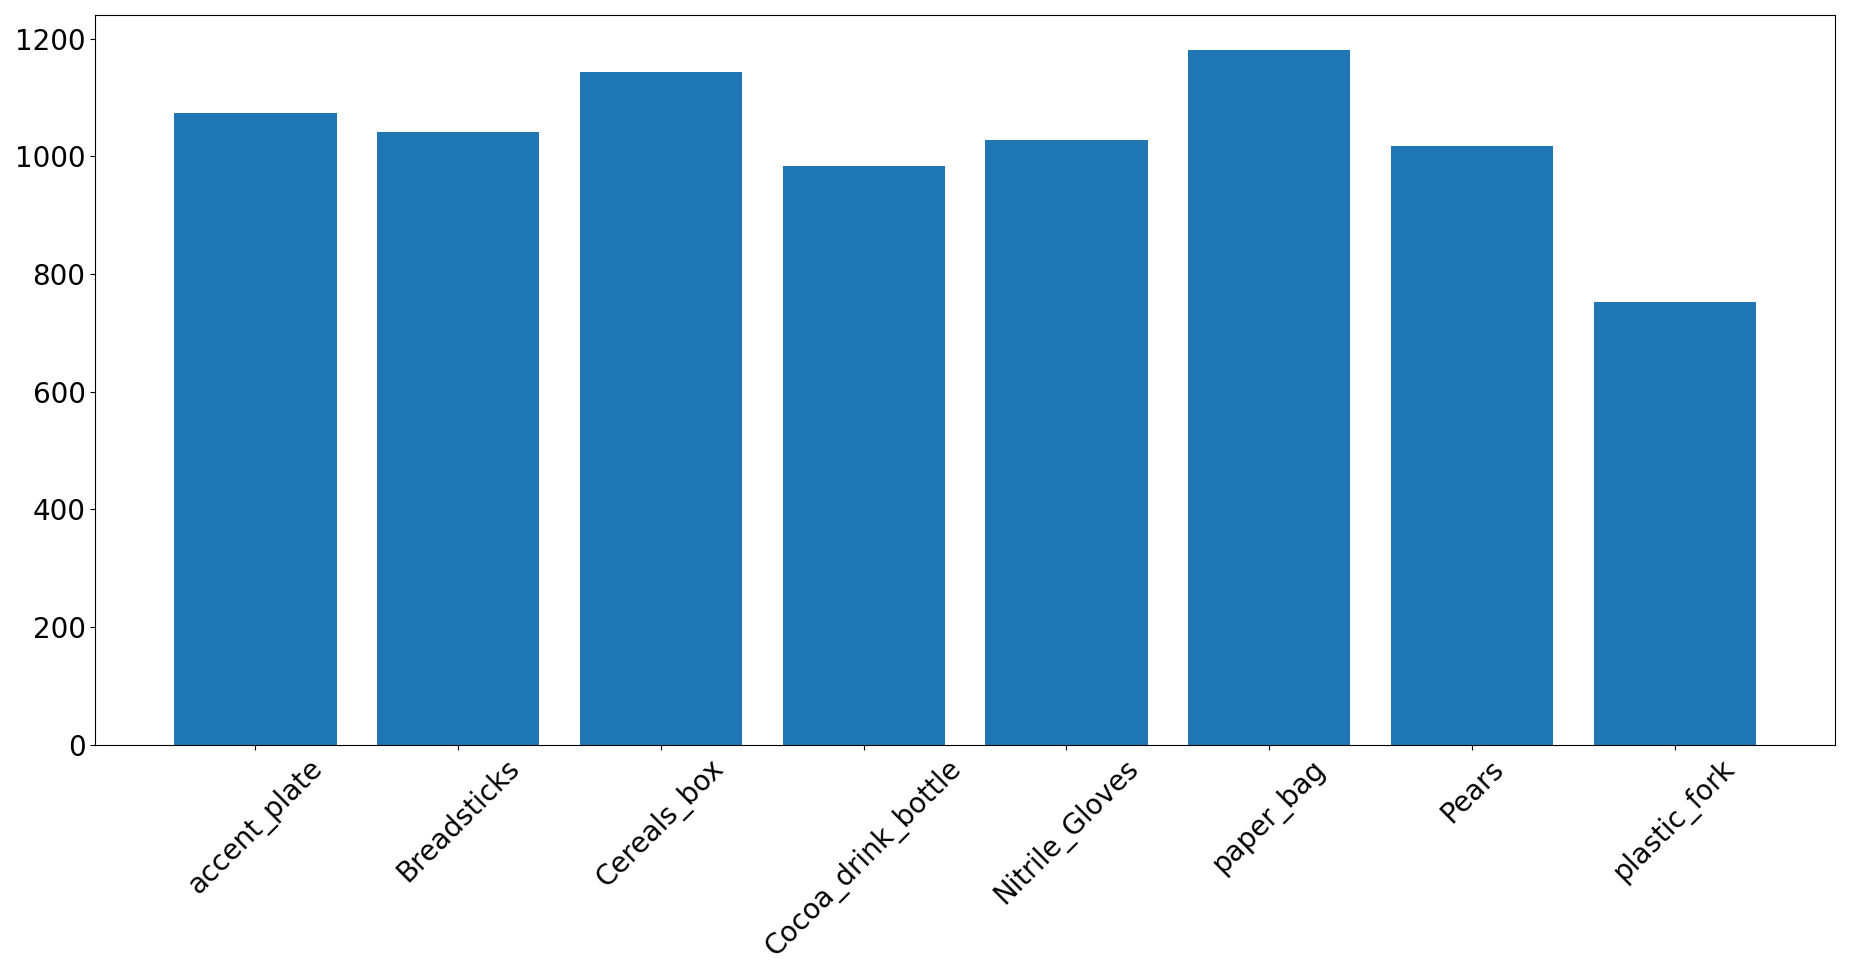
\includegraphics[width=\textwidth]{assets/dataset.png}
		\caption{Distribution of the dataset's 8 classes}
		\label{fig:dataset-distribution}
	\end{figure}

	\noindent
	As we can see in \autoref{fig:dataset-distribution}, the dataset is quite balanced,
	but it should be noted that it also contains outliers -- i.e. misclassified images --
	meaning that our model should adapt accordingly.

	\begin{figure}[H]
		\centering
		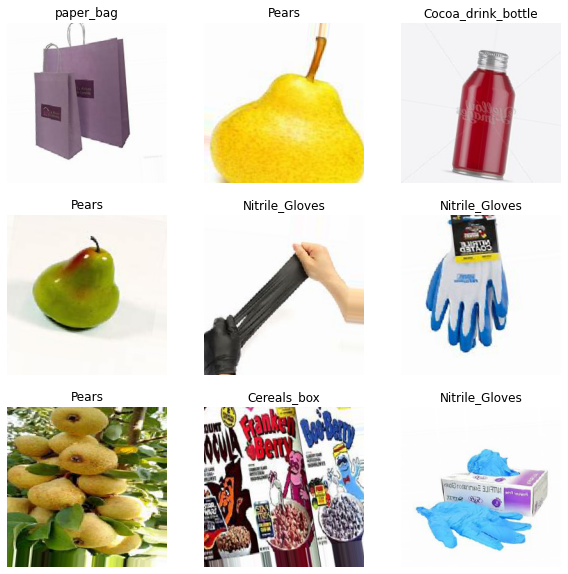
\includegraphics[width=\textwidth]{assets/dataset_samples.png}
		\caption{10 random samples from the dataset}
	\end{figure}



	\section{Preprocessing}
	The first thing I did is the dataset splitting in two subsets for training
	and validation, respectively 70\% and 30\% of the original one.
	The splitting has been made at filesystem level, obtaining two directories
	(\textit{train} and \textit{val}) with the same structure of the original
	one (i.e. with 8 subdirectories, one for each class).


	\subsection{Data augmentation}
	Data augmentation includes techniques used to generate \textit{new} training
	samples from the original ones by applying random jitters and transformations,
	but at the same time ensuring that the class labels of the data are not changed.
	These kind of techniques are useful to reduce overfitting and they usually provide
	an increase in testing accuracy, at the expense of a slight worsening in training accuracy.
	In our case I obtained an increase in the performance by 5 to 10\% applying
	flipping, rotations and zooming to the training set of images.



	\section{Convolutional Neural Networks}
	All the tested solutions for this problem are based on a \textbf{Convolutional Neural Network} (CNN),
	commonly composed by convolutional layers, pooling layers and fully-connected layers.
	The \textbf{convolutional layers} apply a convolution operation to the input images,
	the \textbf{pooling layer} consequently perform a down-sampling through a non linear
	function and the \textbf{fully connected layers} finally classify in one of the 8 classes.


	\subsection{AlexNet}
	The first tested network is the implementation of AlexNet, a popular CNN,
	which has eight layers using the non-saturating \texttt{ReLU} activation function:
	\begin{itemize}
		\item five convolutional layers, some of them followed by a max-pooling layer
		\item three fully connected layers, each one followed by a Dropout layer
	\end{itemize}

	\begin{figure}[H]
		\centering
		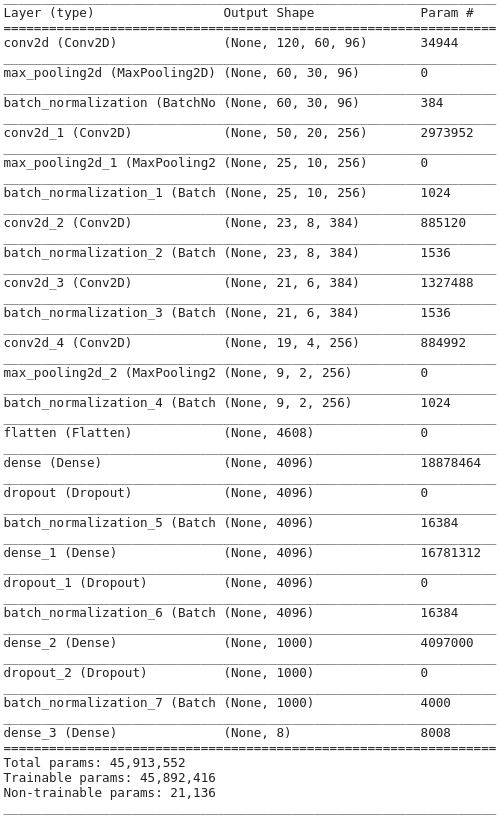
\includegraphics[width=.8\textwidth]{assets/AlexNet.png}
		\caption{Summary of AlexNet}
	\end{figure}


	\subsection{Custom network}
	After the evaluation of AlexNet, the main analysis has been made with a custom
	network, in which it was possible to test different layers and hyperparameters.
	For example adding dropout layers or changing the dropout rate.
	The optimal configuration obtained is showed in \autoref{fig:custom-network-summary},
	all of them using the \texttt{ReLU} activation function except for the last one with \texttt{softmax}

	\begin{figure}[H]
		\centering
		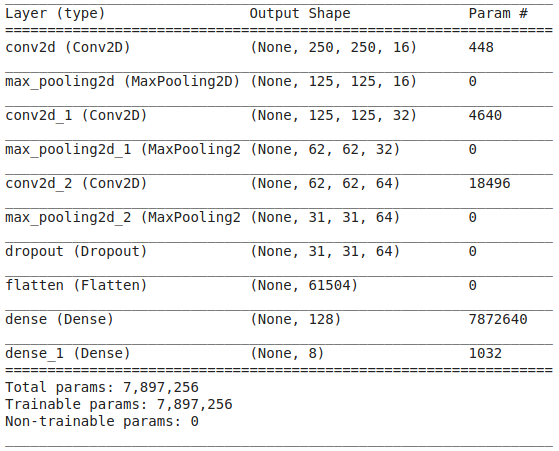
\includegraphics[width=\textwidth]{assets/custom_network.png}
		\caption{Summary of the custom network}
		\label{fig:custom-network-summary}
	\end{figure}



	\section{Evaluation}
	After some test with different epochs values I fixed it at 20 for the final
	evaluation, which was the optimal value for performance and training time.
	To compare the results, in this section are available the accuracy and loss
	curves and also the classification report for both AlexNet and the custom network.
	The accuracy curve shows how the network accuracy increase over every epoch,
	while the loss curve shows how the loss decrease (hopefully).


	\subsection{AlexNet}
	As we can see in \autoref{fig:alexnet-curves}, while the accuracy of the
	training increase and the loss decrease for every epoch, the validation
	results are very poor. The gap between the training curve and the validation
	curve also measure how much our model is prone to overfitting (the model
	adapt too much on the data in the training while performing poor on the overall data available).

	\begin{figure}[H]
		\centering
		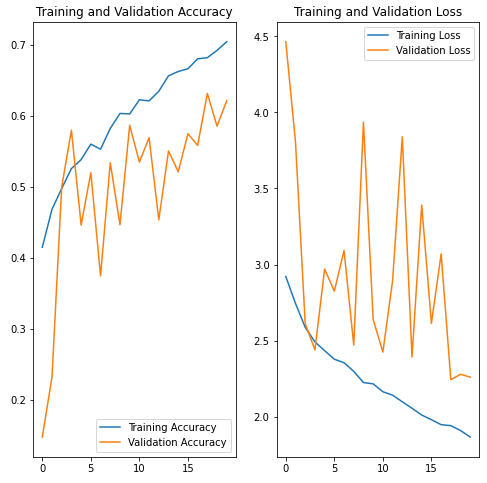
\includegraphics[width=.8\textwidth]{assets/AlexNet_plots.png}
		\caption{AlexNet accuracy and loss plots}
		\label{fig:alexnet-curves}
	\end{figure}

   \begin{table}[H]
		\centering	
		\begin{tabular}{c|c|c|c|c}
			\hline
			& \textbf{Precision} & \textbf{Recall} & \textbf{F1-score} & \textbf{Support} \\
			\hline
			\textit{breadsticks} & 0.776 & 0.674 & 0.721 & 313 \\
			\textit{cereals box} & 0.863 & 0.584 & 0.697 & 344 \\
			\textit{cocoa drink bottle} & 0.554 & 0.449 & 0.496 & 296 \\
			\textit{nitrile gloves} & 0.738 & 0.628 & 0.678 & 309 \\
			\textit{pears} & 0.596 & 0.758 & 0.668 & 306 \\
			\textit{accent plate} & 0.585 & 0.258 & 0.358 & 322 \\
			\textit{paper bag} & 0.812 & 0.293 & 0.431 & 355 \\
			\textit{plastic fork} & 0.239 & 0.850 & 0.373 & 226 \\
			\hline
			\multicolumn{5}{c}{} \\
			\hline
			\textbf{Accuracy} & & & 0.546 & 2471 \\
			\textbf{Macro avg} & 0.645 & 0.562 & 0.553 & 2471 \\
			\textbf{Weighted avg} & 0.666 & 0.546 & 0.558 & 2471 \\
			\hline
		\end{tabular}
		\caption{Classification report of AlexNet}
	\end{table}


	\subsection{Custom network}
	The following results for the custom network are based on the configuration
	with a dropout rate of 0.4, which is the optimal one compared to other values.
	The performance has been increased and regularized compared to the AlexNet ones
	that were unbalanced in precision and recall (e.g. the \textit{plastic fork} class
	had a low precision of 0.239 and a high recall of 0.850).

	\begin{figure}[H]
		\centering
		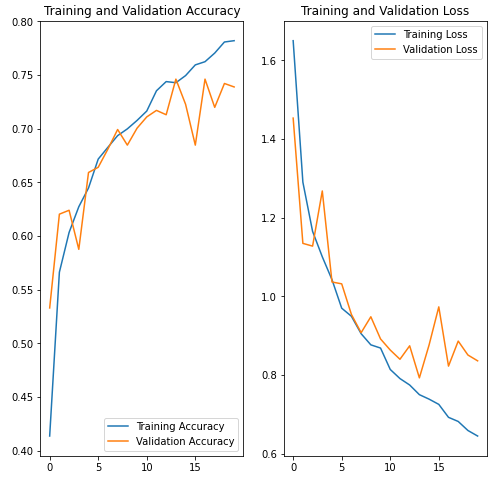
\includegraphics[width=.8\textwidth]{assets/custom_network_plots.png}
		\caption{Custom network accuracy and loss plots}
	\end{figure}

	\begin{table}[H]
		\centering	
		\begin{tabular}{c|c|c|c|c}
			\hline
			& \textbf{Precision} & \textbf{Recall} & \textbf{F1-score} & \textbf{Support} \\
			\hline
			\textit{breadsticks} & 0.816 & 0.693 & 0.750 & 313 \\
			\textit{cereals box} & 0.612 & 0.872 & 0.719 & 344 \\
			\textit{cocoa drink bottle} & 0.569 & 0.514 & 0.540 & 296 \\
			\textit{nitrile gloves} & 0.722 & 0.799 & 0.759 & 309 \\
			\textit{pears} & 0.724 & 0.788 & 0.754 & 306 \\
			\textit{accent plate} & 0.797 & 0.770 & 0.784 & 322 \\
			\textit{paper bag} & 0.711 & 0.507 & 0.592 & 355 \\
			\textit{plastic fork} & 0.651 & 0.602 & 0.652 & 226 \\
			\hline
			\multicolumn{5}{c}{} \\
			\hline
			\textbf{Accuracy} & & & 0.696 & 2471 \\
			\textbf{Macro avg} & 0.700 & 0.693 & 0.690 & 2471 \\
			\textbf{Weighted avg} & 0.702 & 0.696 & 0.692 & 2471 \\
			\hline
		\end{tabular}
		\caption{Classification report of the custom network}
	\end{table}



	\section{Conclusions}
	The performances have been unexpectedly better with the final custom network compared
	to AlexNet, as highlighted by the accuracy and loss curves. The more likely reason
	is that a network like this needs to have a larger dataset and a bigger number
	of epochs to obtain good results. In fact I got better results with 100 epochs,
	but that required more than 1 hour of training.

\end{document}